\section{Convex Hull}
\subsection{Problem Statement}
\begin{itemize}
    \item Implement Quickhull and Graham Scan algorithm to find the convex hull of 2D points. 
    \item Visualize the input 2D points and the convex hull boundary. 
    \item Compare Quickhull and Graham Scan based on various input size on randomly
        generated points.  The comparison metric should be the execution time of 
        each sorting algorithm.
\end{itemize}
\subsection{Code}
\begin{code}
    \caption{generate\_points.cpp}
    \cppcode{../generate_points.cpp}
    \label{code:points}
\end{code}
\begin{code}
    \caption{quick\_hull.cpp}
    \cppcode{../quickhull.cpp}
    \label{code:quickhull}
\end{code}

\begin{code}
    \caption{graham\_scan.cpp}
    \cppcode{../graham_scan.cpp}
    \label{code:graham}
\end{code}
\begin{code}
    \caption{Makefile}
\begin{minted}[
linenos=true,
fontfamily=tt,
fontsize=\small,
linenos=true,
numberblanklines=true,
breaklines=true,
numbersep=5pt,
gobble=0,
frame=leftline,
framerule=0.4pt,
framesep=2mm,
funcnamehighlighting=true,
tabsize=4,
obeytabs=false,
mathescape=false
samepage=false, %with this setting you can force the list to appear on the same page
showspaces=false,
showtabs =false,
texcl=false
    ]{make}
CC=g++

convex: points graham quick

points: generate_points.cpp
	$(CC) $^ -o points.out
	./points.out
graham:	graham_scan.cpp
	$(CC) $^ -o graham_scan.out
	./graham_scan.out

quick: quickhull.cpp
	$(CC) $^ -o quickhull.out
	./quickhull.out

clean:
	rm *.out
    \end{minted}
\end{code}


\begin{code}
    \caption{visualization.py}
    \begin{minted}[
linenos=true,
fontfamily=tt,
fontsize=\small,
linenos=true,
numberblanklines=true,
breaklines=true,
numbersep=5pt,
gobble=0,
frame=leftline,
framerule=0.4pt,
framesep=2mm,
funcnamehighlighting=true,
tabsize=4,
obeytabs=false,
mathescape=false
samepage=false, %with this setting you can force the list to appear on the same page
showspaces=false,
showtabs =false,
texcl=false
    ]{python}
import matplotlib.pyplot as plt 
%matplotlib inline
X = [ 44, 63, 90, 43, 54, 26, 42, 47, 57, 2, 61, 72, 24, 88, 82, 78, 33, 74, 55, 19, 99, 24, 42, 73, 18, 32, 41, 43, 64, 49, 8, 73, 66, 13, 66, 32, 27, 8, 82, 69, 5, 80, 59, 12, 56, 70, 86, 7, 40, 74, 54, 20, 65, 51, 59, 96, 76, 60, 100, 60, 83, 75, 23, 22, 4, 18, 57, 89, 16, 18, 11, 90, 43, 71, 24, 1, 11, 78, 60, 46, 51, 72, 51, 79, 100, 93, 12, 99, 82, 47, 51, 64, 26, 97, 92, 100, 56, 100, 31, 24 ]
Y = [ 55, 98, 64, 46, 32, 64, 98, 29, 44, 83, 16, 14, 57, 82, 26, 77, 40, 22, 68, 61, 44, 93, 23, 50, 74, 30, 55, 16, 83, 97, 26, 92, 46, 72, 31, 64, 8, 20, 80, 99, 53, 97, 74, 74, 60, 16, 42, 3, 72, 5, 58, 80, 28, 46, 72, 64, 27, 34, 24, 8, 29, 20, 33, 62, 48, 58, 37, 21, 40, 75, 65, 86, 49, 94, 30, 7, 27, 33, 52, 63, 63, 7, 61, 67, 96, 62, 82, 54, 69, 6, 100, 13, 41, 85, 42, 42, 71, 6, 78, 82 ]
x = [ 100, 69, 51, 42, 24, 2, 1, 7, 74, 100, 100 ]
y = [ 96, 99, 100, 98, 93, 83, 7, 3, 5, 6, 96]

plt.scatter(X,Y, label="n=100")
plt.plot(x,y,color="red")
plt.xlabel("x") 
plt.ylabel("y")
plt.legend()
plt.savefig("convex_100pt.png", dpi=300, bbox_inches="tight")
    \end{minted}
\end{code}

\subsection{Output}

\begin{figure}[H]
    \centering
    \begin{subfigure}[b]{0.4\textwidth}
        \centering
        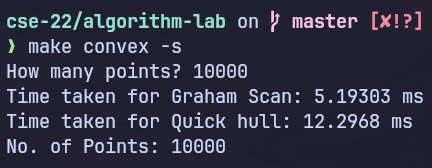
\includegraphics[width=\textwidth]{./img/lab2/p10k.png}
        \caption{Execution time for n=$10^4$}
    \end{subfigure}
    \hfill
    \begin{subfigure}[b]{0.4\textwidth}
        \centering
        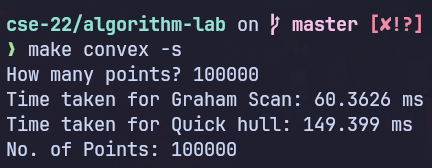
\includegraphics[width=\textwidth]{./img/lab2/p100k.png}
        \caption{Execution time for n=$10^5$}
    \end{subfigure}
    \hfill
    \begin{subfigure}[b]{0.4\textwidth}
        \centering
        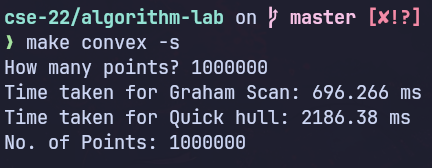
\includegraphics[width=\textwidth]{./img/lab2/p1000k.png}
        \caption{Execution time for n=$10^6$}
    \end{subfigure}
    \hfill
    \begin{subfigure}[b]{0.4\textwidth}
        \centering
        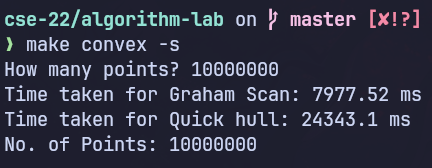
\includegraphics[width=\textwidth]{./img/lab2/p1cr.png}
        \caption{Execution time for n=$10^7$}

    \end{subfigure}
    \caption{Convex hull algorithm execution time}
    \label{fig:task1}

\end{figure}

\subsubsection*{Summary of Execution time}
\begin{table}[H]
    \centering
    \caption{Comparison table for Graham Scan \& Quick Hull algorithm execution time}
    \label{tab:comp}
    \begin{tabular}{lSS}
        \toprule
        \multicolumn{1}{c}{Input Size} & \multicolumn{1}{c}{Graham Scan (ms)} & \multicolumn{1}{c}{Quick Hull (ms)} \\
        \midrule
        $10^3$   & 0.440 & 1.000 \\
        $5\times 10^3$   & 2.385  & 5.553 \\
        $10^4$  & 5.193  & 12.297 \\
        $5\times 10^4$  & 30.383 & 81.619\\
        $10^5$ & 60.363  & 149.399  \\
        $10^6$ & 696.266 & 2186.380 \\
        $10^7$ & 7977.520 & 24343.100 \\
        \bottomrule
    \end{tabular}
\end{table}
\begin{figure}[H]
    \centering
    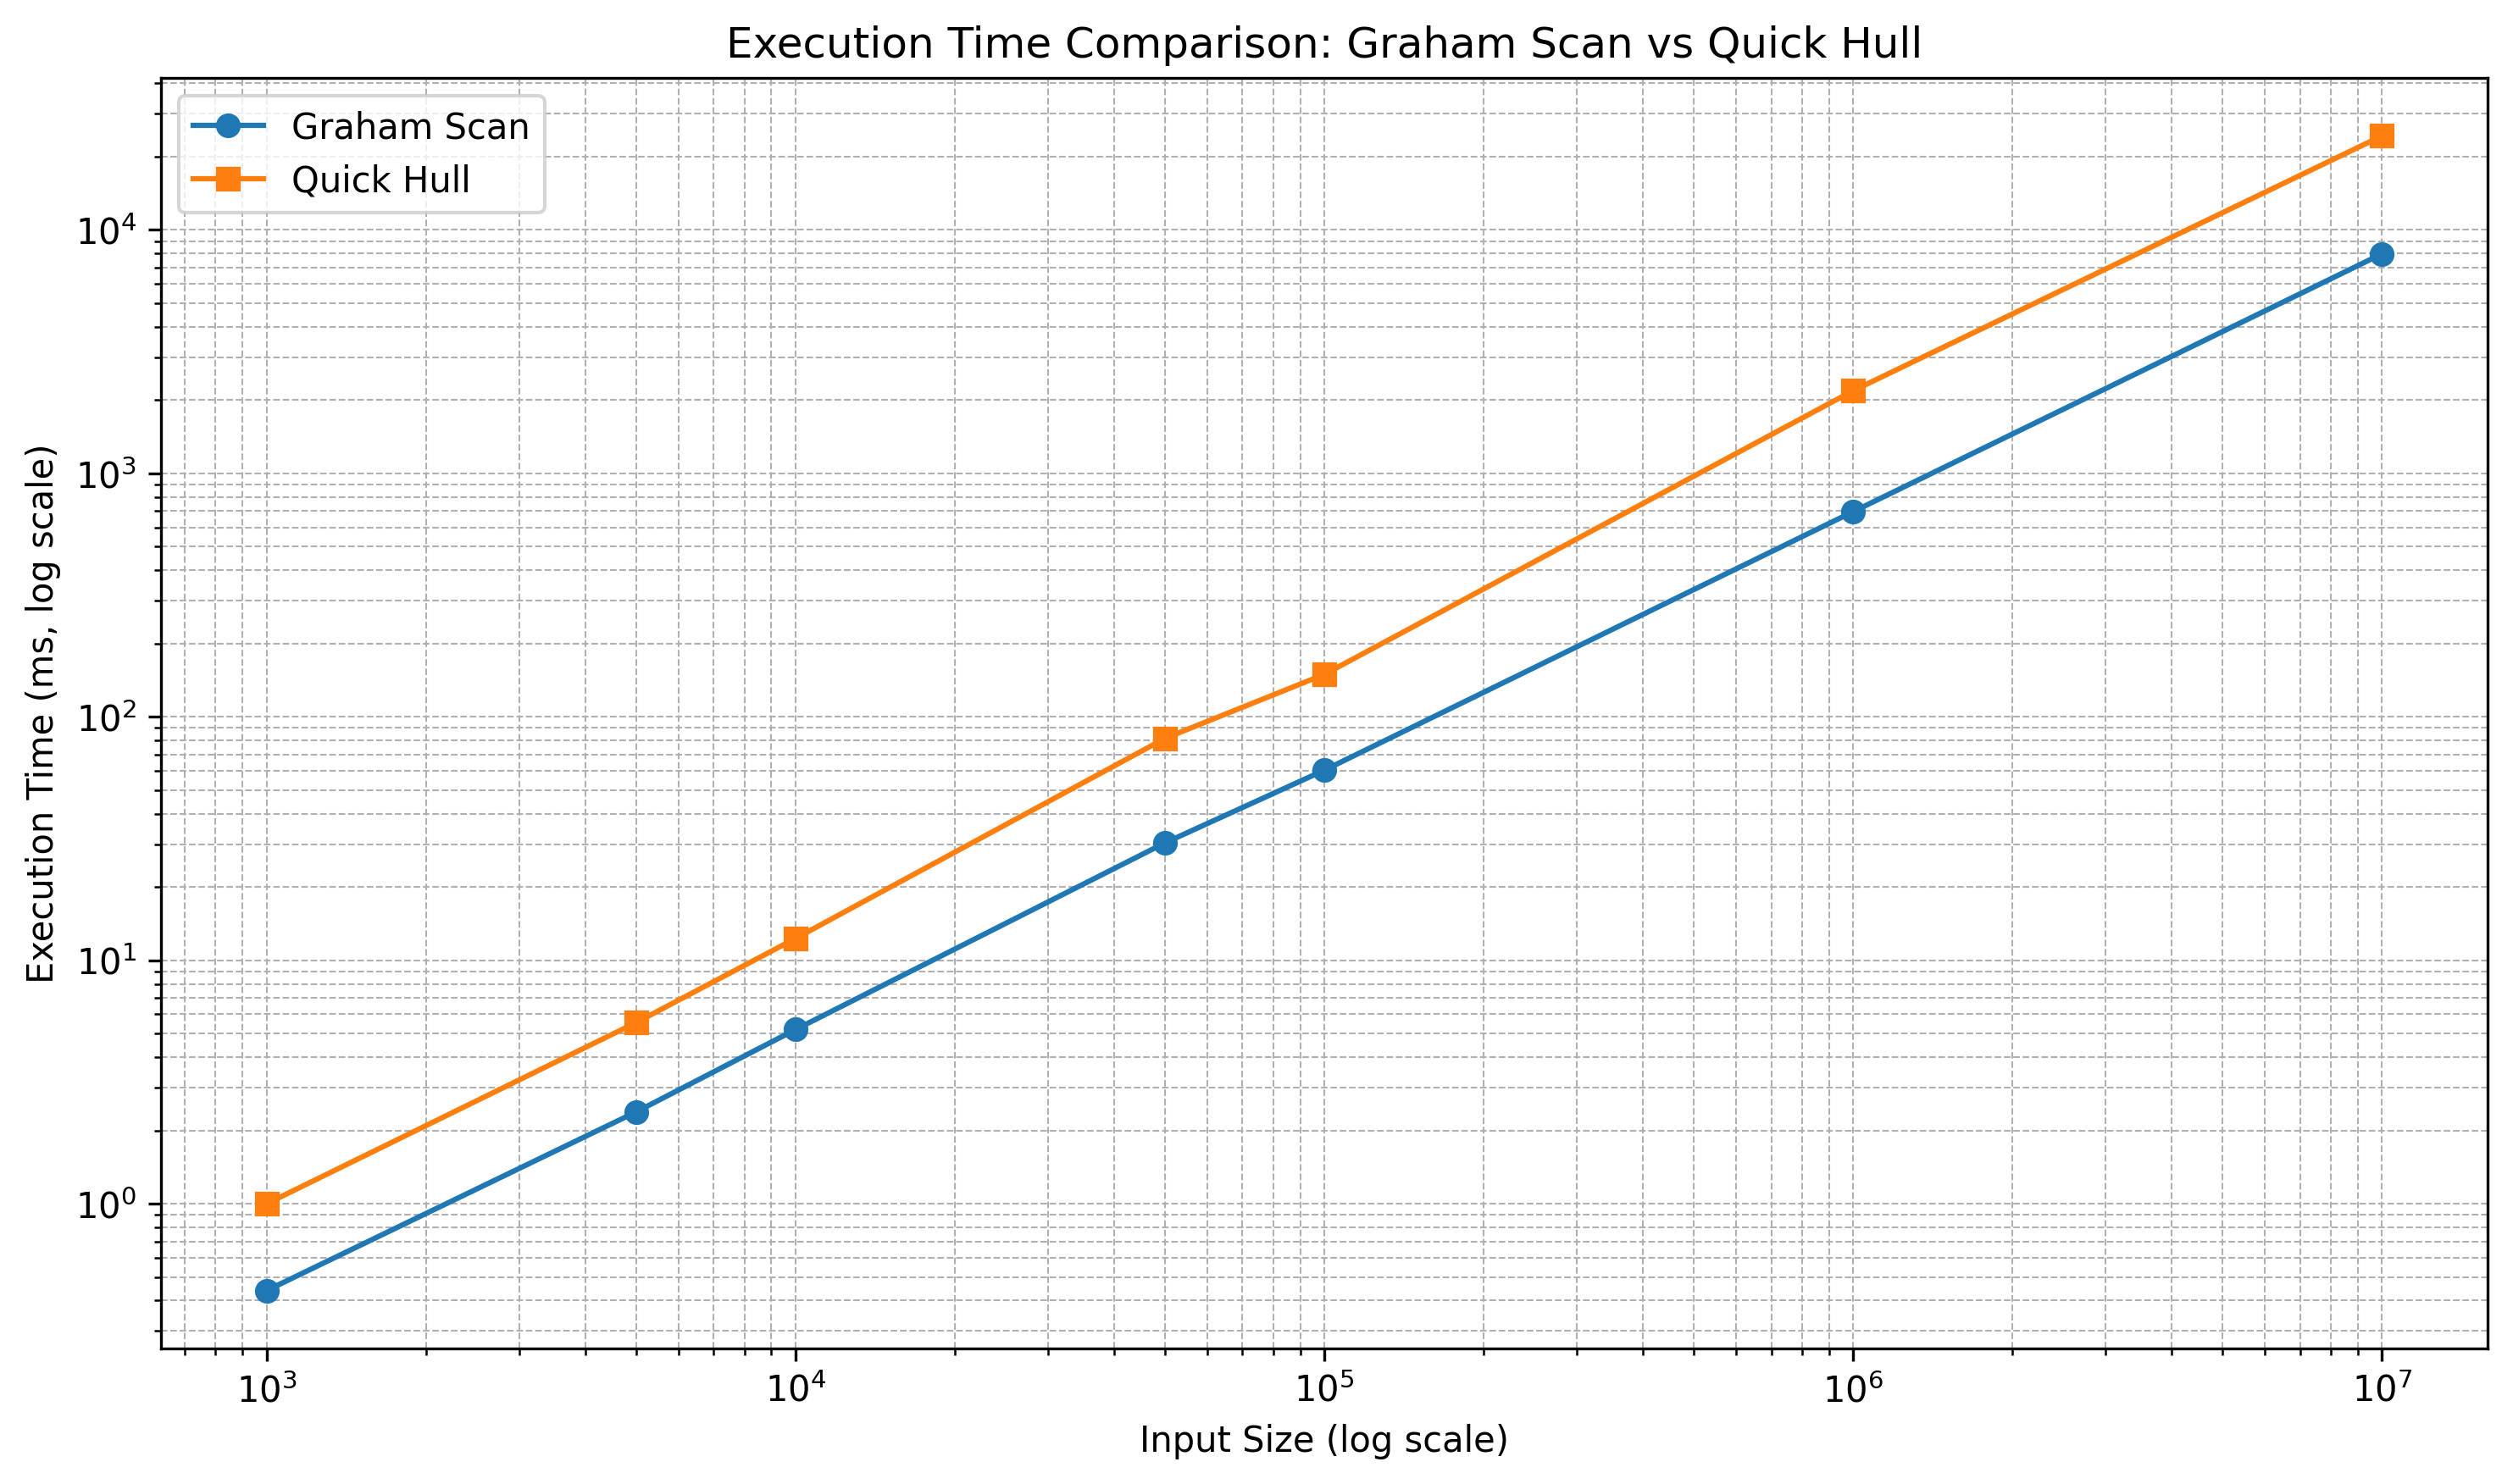
\includegraphics[width=\textwidth]{img/lab2/comparison_plot.png}
    \caption{Execution time comparison}
    \label{fig:comp}
\end{figure}
\subsubsection*{Visualization}

\begin{figure}[H]
    \centering
    \begin{subfigure}[b]{0.5\textwidth}
        \centering
        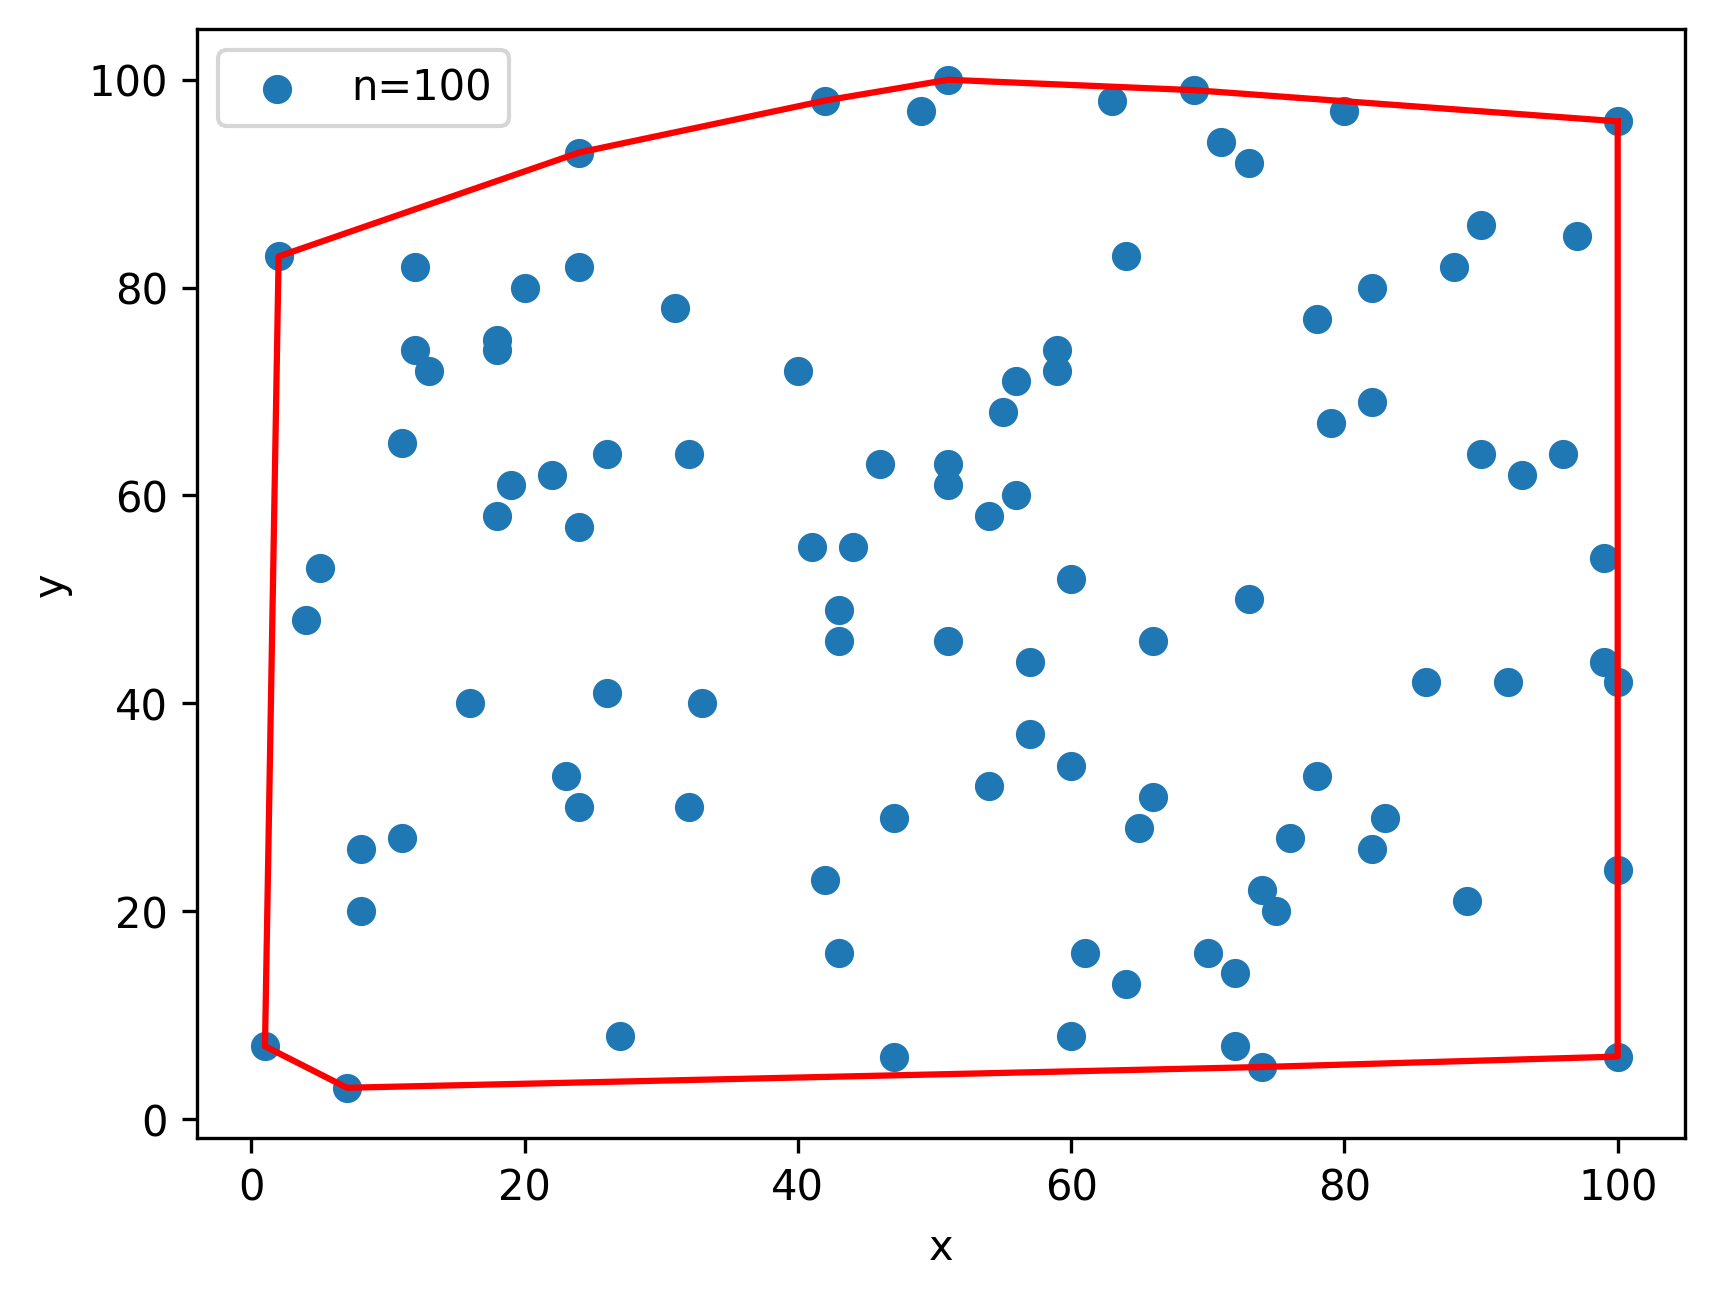
\includegraphics[width=\textwidth]{./img/lab2/convex_100pt.png}
        \caption{Convex hull visualization using graham scan for 100 points}
    \end{subfigure}
    \hfill
    \begin{subfigure}[b]{0.5\textwidth}
        \centering
        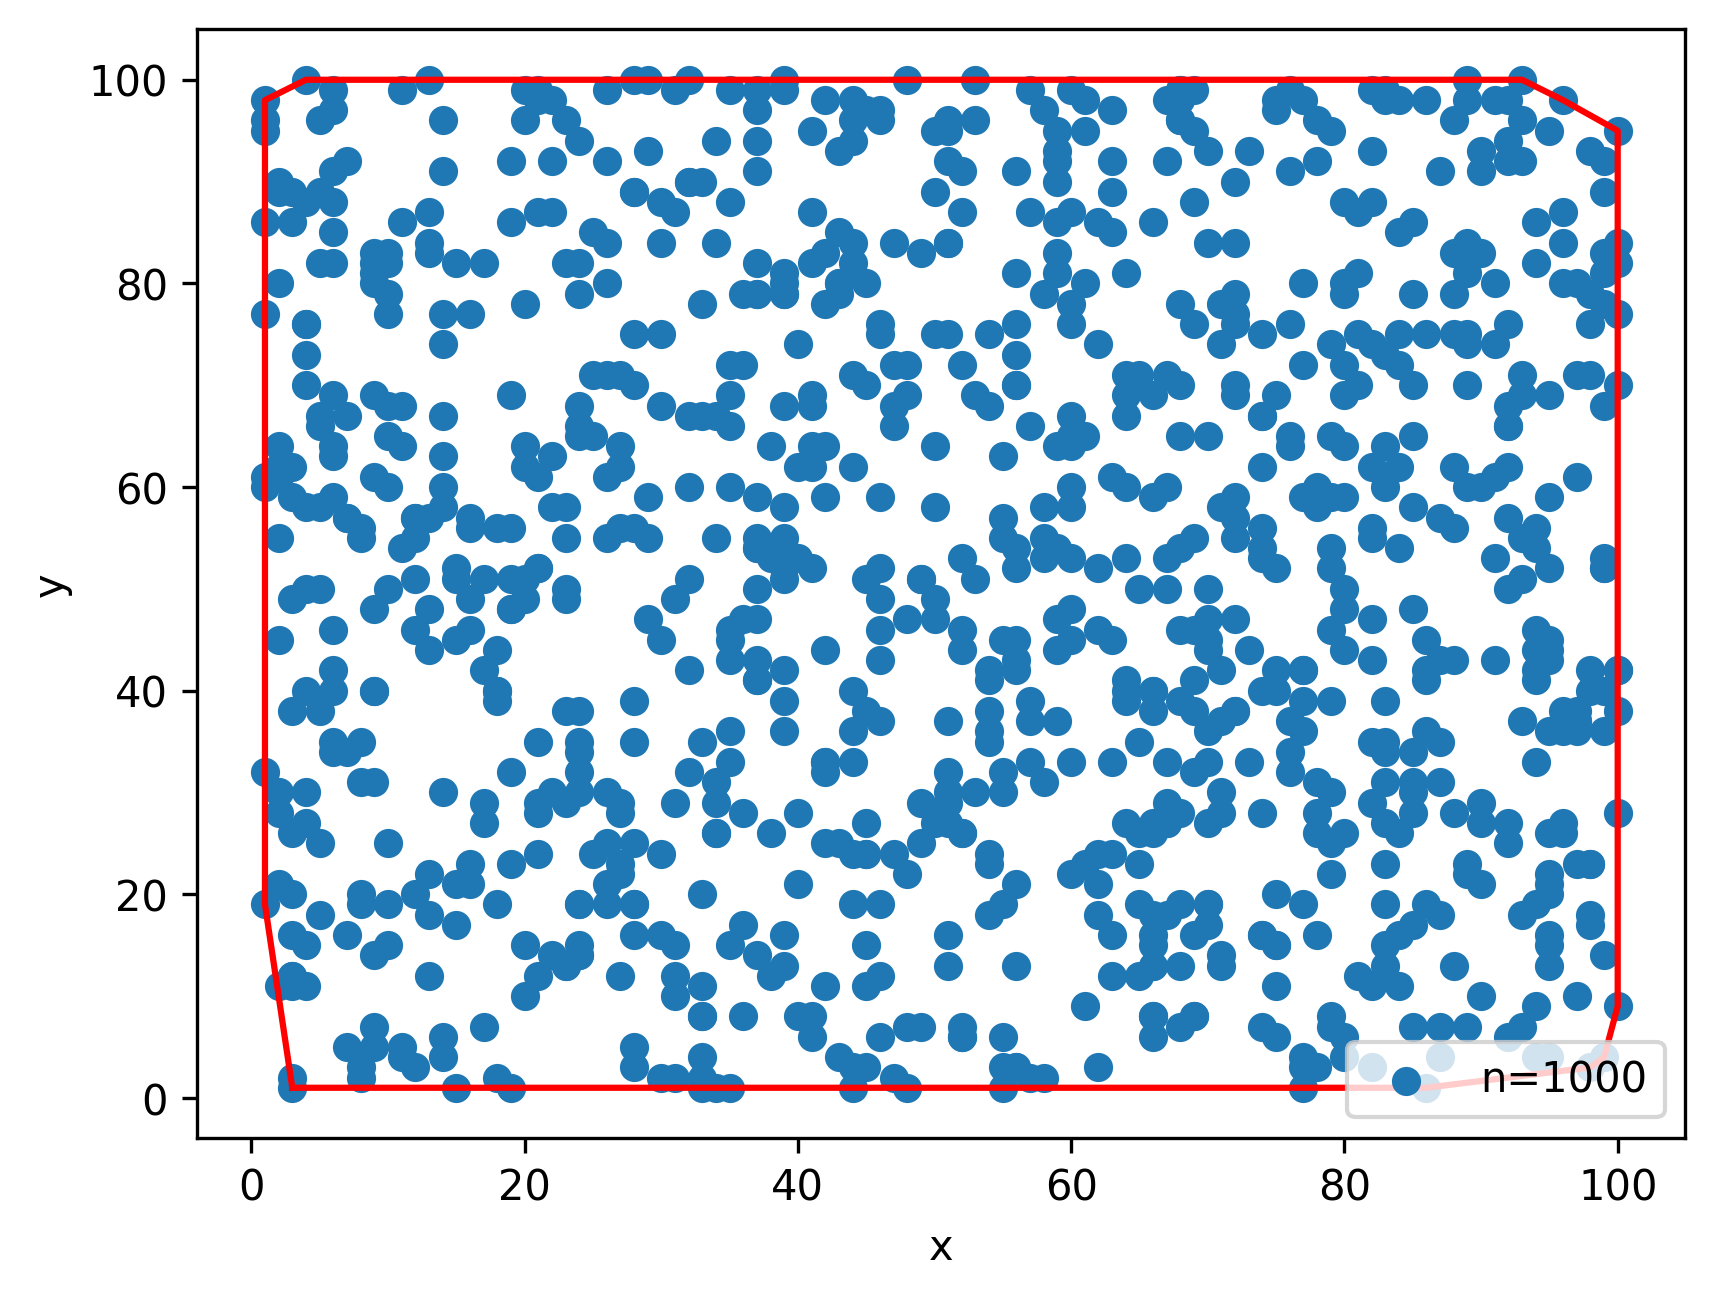
\includegraphics[width=\textwidth]{./img/lab2/convex_1kpt.png}
        \caption{Convex hull visualization using quick hull for 1000 points}
    \end{subfigure}
    
    \caption{Convex hull Visualization}
    \label{fig:task2}
\end{figure}
\subsection{Analysis \& Discussion}
The implemented code sucessfully finds the convex hull points using
Graham scan and Quick hull algorithms (see \cref{fig:task2}). In case of
execution time, from the comparison \cref{tab:comp} and \cref{fig:comp}
it is clear that Graham scan
outperforms quick hull for any input size. With increasing number of input sizes
Graham scan is almost 3 times faster than quick hull.

This is because Graham scan has $O(n \log n)$ complexity for any input size. 
Whereas Quick Hull algorithm uses a divide and conquer approach having the 
the complexity of $O(n \log n)$ for avarage case and $O(n^2)$ in worst case.

Graham scan always sorts the points in polar angle order. This step takes the 
largest cost. More efficient algorithm for sorting can also imporve this step's 
complexity. 

In conclusion, Graham scan is more efficent in comparison to quick hull. Also
the simplicity in implementation for Graham scan is much more
preferred over quick
hull algorithm.

